%AXIOMATIC MODEL DEMYSTIFIED----------------------------------------------

\documentclass[10pt]{article}
\usepackage[utf8]{inputenc}
\usepackage{amsmath}
\usepackage{amssymb}
\usepackage{geometry}
\usepackage[dvipsnames]{xcolor}
\usepackage{graphicx}
\usepackage{tikz}
\usepackage{amsthm}
\usepackage{float}
\usepackage{centernot}
\usepackage{tasks}

\title{ECMAScript Axiomatic Memory Consistency Model}
\author{Akshay Gopalakrishnan}
\date{November 2019}

%Short form to use stack_relative
\newcommand{\stck}{\stackrel{\longrightarrow}}

%A different version of the above 
\newcommand{\stckdet}[1]{\stackrel{{#1}}}

%We write a lot of relations between two events using the orderings, so a short form to use that
\newcommand{\reln}[3]{#1\stck{_{#2}}#3}

%We use a more detailed version of the above relation to indicate direct / indirect relations 

\newcommand{\reldet}[4]{#1\stckdet{_{#2}}{{\stck{_{#3}}}}#4}

%We also will introduce a short form to write an event belongs to some set
\newcommand{\event}[2]{#1\!\in\!#2}

%To make events and their type more close to each other
\newcommand{\typ}[1]{\textit{#1}}
\newcommand{\et}[2]{#1\!:\!\typ{#2}}

%Short form to write color text
\newcommand{\critic}[2]{\textcolor{#1}{\footnotesize #2}}

%A new command to quickly use cons function in formal descriptions
\newcommand{\cons}[2]{\textit{cons}(#1,#2)}

%Useful command syntax
\newcommand{\rmw}{\textit{rmw}\,}
\newcommand{\set}[1]{\textbf{\textit{#1}}}

%Some preliminary latex commands to format writing theorems 
\newtheorem{lemma}{Lemma}

\newtheorem{theorem}{Theorem}[lemma]

\newtheorem{corollary}{Corollary}[theorem]

\newtheorem{definition}{Definition}

\newtheorem{property}{Property}


\begin{document}

    \maketitle

    %
\section{Introduction}
    Instruction reordering is a common transformation done by the compiler/hardware, which is essential to optimizations such as instruction scheduling, loop invariant removal, partial redundancy elimination, etc. 
    However, whether we can do such reordering freely given a concurrent program using relaxed memory accesses is a bit unclear. 
     
    \paragraph{Simple reordering is not straightforward under shared memory semantics}
    The main reason is that memory accesses here, do not just perform the desired operation (i.e Read / Write) but also imply certain visibility guarantees across all the other threads.  
    In our observation, we find that, the relaxed memory model of ECMAScript prescribe semantics for visibility using the $\stck{_{hb}}$ relations. 
    
    \paragraph{Some Examples}
        We show a couple of examples to showcase why reordering may not be that straightforward. 
        Consider the first example in Figure~\ref{reord:example1(a)} below of a Candidate before and after reordering two events.
        The original candidate is to the left and that on the right is after reordering the two reads of $T2$.
        The observable behavior in question is written in the middle(orange box). 
        \begin{figure}[H]
            \centering
            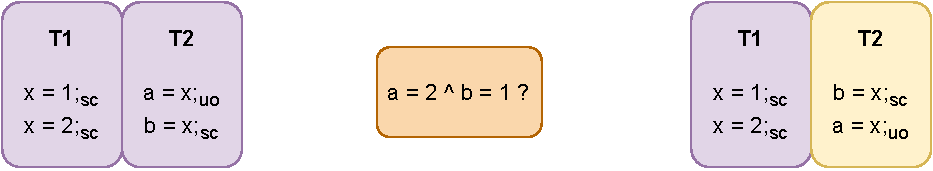
\includegraphics[scale=0.7]{5.InstructionReordering/0.Intro/ReorderingExample1(a).pdf}
            \caption{First example for reordering in candidates of the original program and its reordered counterpart.}
            \label{reord:example1(a)} 
        \end{figure}
        
        Figure~\ref{reord:example1(b)} has two sets of relations. 
        The first justifies the outcome for the reordered Candidate. 
        While the second justifies for the original Candidate. 
        Notice that in the first set of relations, we can infer that one may have a read memory ordered before a write that it reads from. 
        This is quite counter intuitive to understand at first. 
        But strictly from the semantics of the model, this justification to the observable behavior is completely valid\footnotemark. 
        \begin{figure}[H]
            \centering
            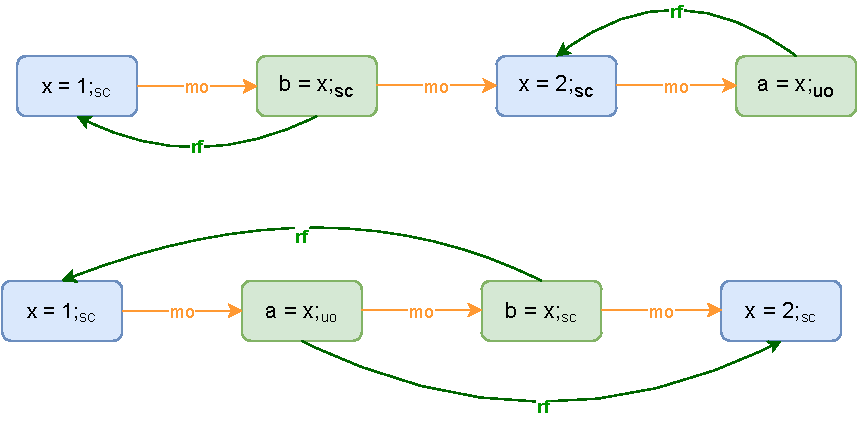
\includegraphics[scale=0.7]{5.InstructionReordering/0.Intro/ReorderingExample1(b).pdf}
            \caption{The set of partial order relations justifying the observable behavior in question for both the candidates in Figure~\ref{reord:example1(a)}.} 
            \label{reord:example1(b)}
        \end{figure}

        \footnotetext{In practice, this can be due to read speculation at the hardware level.}
        
        Consider another example in Figure~\ref{reord:example2(a)}.
        The figure on the left is the original candidate and that on the right is after reordering the two events of $T1$.
        The observable behavior in question is written in the middle(orange box). 
        \begin{figure}[H]
            \centering
            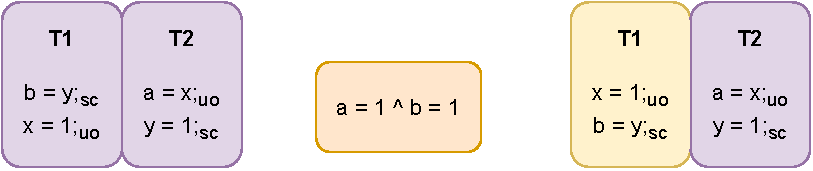
\includegraphics[scale=0.7]{5.InstructionReordering/0.Intro/ReorderingExample2(a).pdf}
            \caption{Second example for reordering with candidates of the original program and its reordered counterpart.} 
            \label{reord:example2(a)}
        \end{figure}
   
        Figure~\ref{reord:example2(b)} has two sets of relations. 
        The first justifies that such an outcome is not possible for the original program candidate due to Axiom \ref{CoRe}. 
        While the second justifies that this outcome is possible for the reordered program.
        Note that we cannot infer in the reordered candidate the set of relations for any candidate execution to have $\reln{a=x;_{uo}}{hb}{x=1;_{uo}}$. 
        \begin{figure}[H]
            \centering
            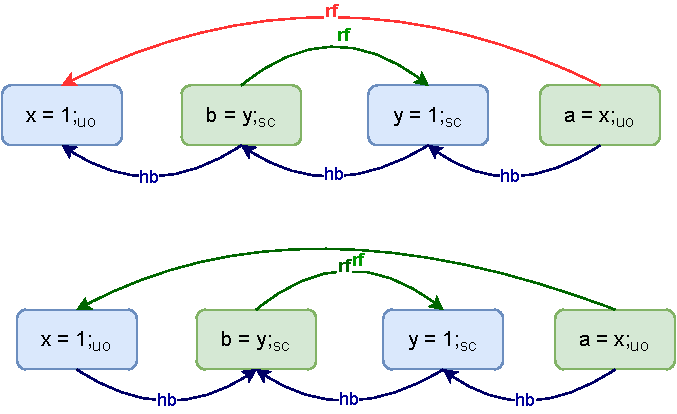
\includegraphics[scale=0.7]{5.InstructionReordering/0.Intro/ReorderingExample2(b).pdf}
            \caption{The set of partial order relations justifying the observable behavior in question for both the candidates in Figure~\ref{reord:example2(a)}.} 
            \label{reord:example2(b)}
        \end{figure}

        The above two examples show that we have to be careful while reordering two events in the same thread. 
        By example analysis, for each observable behavior, one must check all possible candidate executions and assert whether such an observable is possible or not. 
        This method of checking validity of reordering will scale exponentially as the program size increases. 
        It may also be the case that the compiler may not have information on which exact events would be executed in other threads to assert such reordering is valid. 

    
    
    
    
    

    %The ECMAScript Memory Model
    
\section{Introduction}
    Instruction reordering is a common transformation done by the compiler/hardware, which is essential to optimizations such as instruction scheduling, loop invariant removal, partial redundancy elimination, etc. 
    However, whether we can do such reordering freely given a concurrent program using relaxed memory accesses is a bit unclear. 
     
    \paragraph{Simple reordering is not straightforward under shared memory semantics}
    The main reason is that memory accesses here, do not just perform the desired operation (i.e Read / Write) but also imply certain visibility guarantees across all the other threads.  
    In our observation, we find that, the relaxed memory model of ECMAScript prescribe semantics for visibility using the $\stck{_{hb}}$ relations. 
    
    \paragraph{Some Examples}
        We show a couple of examples to showcase why reordering may not be that straightforward. 
        Consider the first example in Figure~\ref{reord:example1(a)} below of a Candidate before and after reordering two events.
        The original candidate is to the left and that on the right is after reordering the two reads of $T2$.
        The observable behavior in question is written in the middle(orange box). 
        \begin{figure}[H]
            \centering
            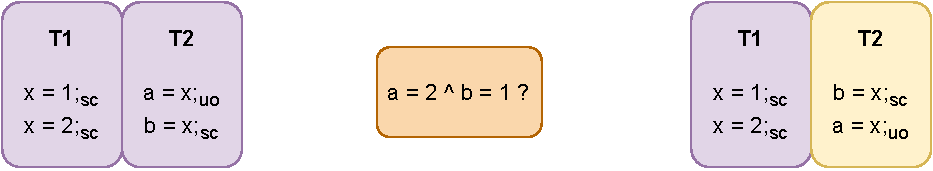
\includegraphics[scale=0.7]{5.InstructionReordering/0.Intro/ReorderingExample1(a).pdf}
            \caption{First example for reordering in candidates of the original program and its reordered counterpart.}
            \label{reord:example1(a)} 
        \end{figure}
        
        Figure~\ref{reord:example1(b)} has two sets of relations. 
        The first justifies the outcome for the reordered Candidate. 
        While the second justifies for the original Candidate. 
        Notice that in the first set of relations, we can infer that one may have a read memory ordered before a write that it reads from. 
        This is quite counter intuitive to understand at first. 
        But strictly from the semantics of the model, this justification to the observable behavior is completely valid\footnotemark. 
        \begin{figure}[H]
            \centering
            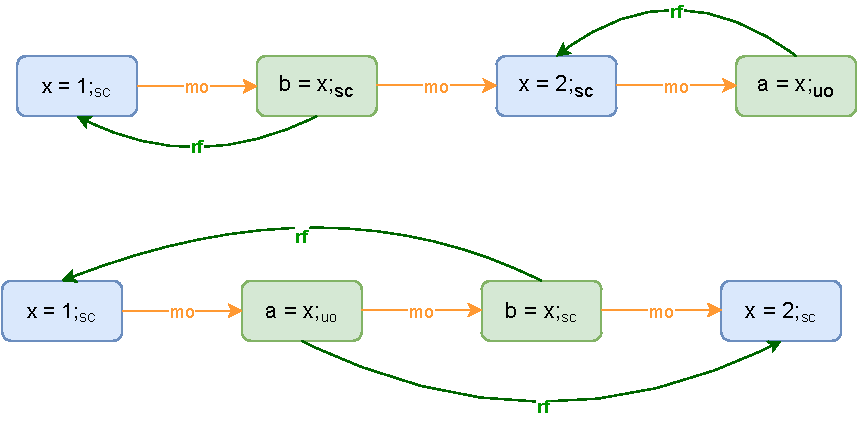
\includegraphics[scale=0.7]{5.InstructionReordering/0.Intro/ReorderingExample1(b).pdf}
            \caption{The set of partial order relations justifying the observable behavior in question for both the candidates in Figure~\ref{reord:example1(a)}.} 
            \label{reord:example1(b)}
        \end{figure}

        \footnotetext{In practice, this can be due to read speculation at the hardware level.}
        
        Consider another example in Figure~\ref{reord:example2(a)}.
        The figure on the left is the original candidate and that on the right is after reordering the two events of $T1$.
        The observable behavior in question is written in the middle(orange box). 
        \begin{figure}[H]
            \centering
            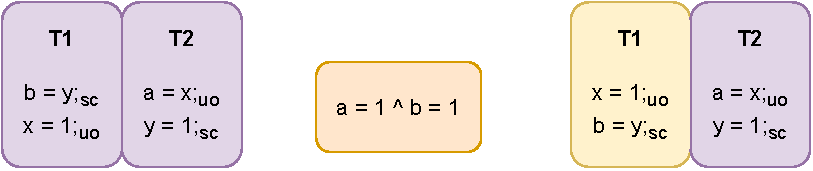
\includegraphics[scale=0.7]{5.InstructionReordering/0.Intro/ReorderingExample2(a).pdf}
            \caption{Second example for reordering with candidates of the original program and its reordered counterpart.} 
            \label{reord:example2(a)}
        \end{figure}
   
        Figure~\ref{reord:example2(b)} has two sets of relations. 
        The first justifies that such an outcome is not possible for the original program candidate due to Axiom \ref{CoRe}. 
        While the second justifies that this outcome is possible for the reordered program.
        Note that we cannot infer in the reordered candidate the set of relations for any candidate execution to have $\reln{a=x;_{uo}}{hb}{x=1;_{uo}}$. 
        \begin{figure}[H]
            \centering
            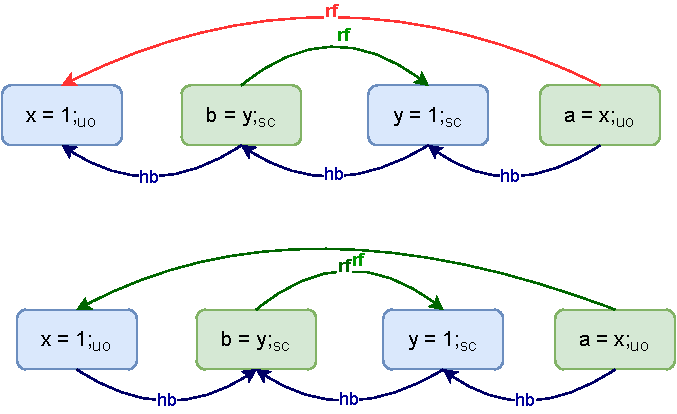
\includegraphics[scale=0.7]{5.InstructionReordering/0.Intro/ReorderingExample2(b).pdf}
            \caption{The set of partial order relations justifying the observable behavior in question for both the candidates in Figure~\ref{reord:example2(a)}.} 
            \label{reord:example2(b)}
        \end{figure}

        The above two examples show that we have to be careful while reordering two events in the same thread. 
        By example analysis, for each observable behavior, one must check all possible candidate executions and assert whether such an observable is possible or not. 
        This method of checking validity of reordering will scale exponentially as the program size increases. 
        It may also be the case that the compiler may not have information on which exact events would be executed in other threads to assert such reordering is valid. 

    
    
    
    
    

    %Instruction reordering
    %\input{InstructionReordering/reordering_opt.tex}

    %Elimination 
    %
\section{Introduction}
    Instruction reordering is a common transformation done by the compiler/hardware, which is essential to optimizations such as instruction scheduling, loop invariant removal, partial redundancy elimination, etc. 
    However, whether we can do such reordering freely given a concurrent program using relaxed memory accesses is a bit unclear. 
     
    \paragraph{Simple reordering is not straightforward under shared memory semantics}
    The main reason is that memory accesses here, do not just perform the desired operation (i.e Read / Write) but also imply certain visibility guarantees across all the other threads.  
    In our observation, we find that, the relaxed memory model of ECMAScript prescribe semantics for visibility using the $\stck{_{hb}}$ relations. 
    
    \paragraph{Some Examples}
        We show a couple of examples to showcase why reordering may not be that straightforward. 
        Consider the first example in Figure~\ref{reord:example1(a)} below of a Candidate before and after reordering two events.
        The original candidate is to the left and that on the right is after reordering the two reads of $T2$.
        The observable behavior in question is written in the middle(orange box). 
        \begin{figure}[H]
            \centering
            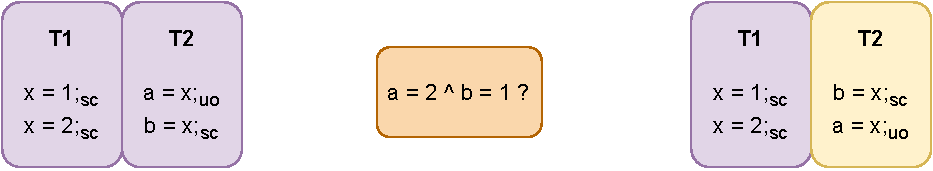
\includegraphics[scale=0.7]{5.InstructionReordering/0.Intro/ReorderingExample1(a).pdf}
            \caption{First example for reordering in candidates of the original program and its reordered counterpart.}
            \label{reord:example1(a)} 
        \end{figure}
        
        Figure~\ref{reord:example1(b)} has two sets of relations. 
        The first justifies the outcome for the reordered Candidate. 
        While the second justifies for the original Candidate. 
        Notice that in the first set of relations, we can infer that one may have a read memory ordered before a write that it reads from. 
        This is quite counter intuitive to understand at first. 
        But strictly from the semantics of the model, this justification to the observable behavior is completely valid\footnotemark. 
        \begin{figure}[H]
            \centering
            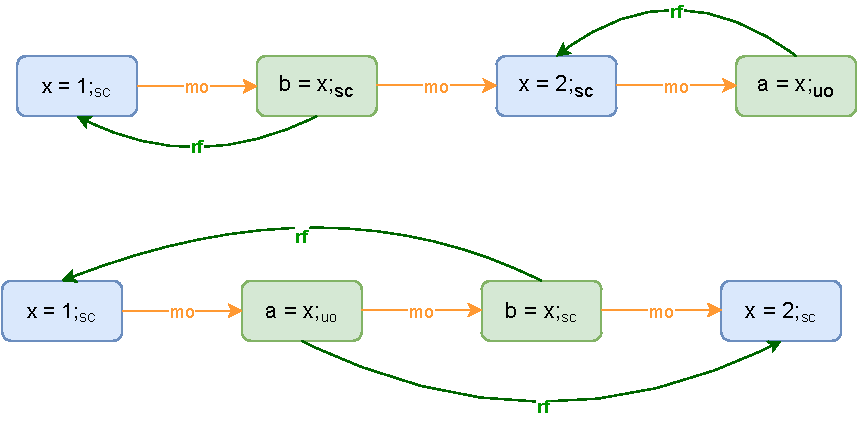
\includegraphics[scale=0.7]{5.InstructionReordering/0.Intro/ReorderingExample1(b).pdf}
            \caption{The set of partial order relations justifying the observable behavior in question for both the candidates in Figure~\ref{reord:example1(a)}.} 
            \label{reord:example1(b)}
        \end{figure}

        \footnotetext{In practice, this can be due to read speculation at the hardware level.}
        
        Consider another example in Figure~\ref{reord:example2(a)}.
        The figure on the left is the original candidate and that on the right is after reordering the two events of $T1$.
        The observable behavior in question is written in the middle(orange box). 
        \begin{figure}[H]
            \centering
            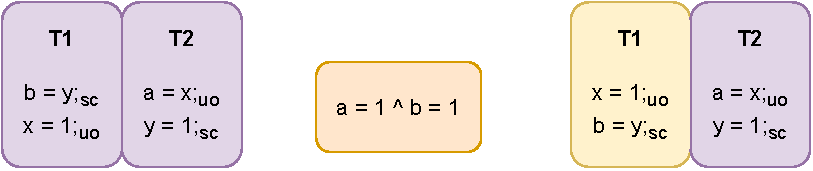
\includegraphics[scale=0.7]{5.InstructionReordering/0.Intro/ReorderingExample2(a).pdf}
            \caption{Second example for reordering with candidates of the original program and its reordered counterpart.} 
            \label{reord:example2(a)}
        \end{figure}
   
        Figure~\ref{reord:example2(b)} has two sets of relations. 
        The first justifies that such an outcome is not possible for the original program candidate due to Axiom \ref{CoRe}. 
        While the second justifies that this outcome is possible for the reordered program.
        Note that we cannot infer in the reordered candidate the set of relations for any candidate execution to have $\reln{a=x;_{uo}}{hb}{x=1;_{uo}}$. 
        \begin{figure}[H]
            \centering
            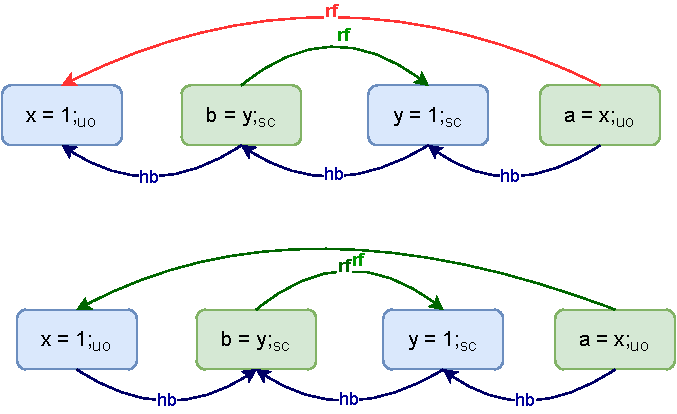
\includegraphics[scale=0.7]{5.InstructionReordering/0.Intro/ReorderingExample2(b).pdf}
            \caption{The set of partial order relations justifying the observable behavior in question for both the candidates in Figure~\ref{reord:example2(a)}.} 
            \label{reord:example2(b)}
        \end{figure}

        The above two examples show that we have to be careful while reordering two events in the same thread. 
        By example analysis, for each observable behavior, one must check all possible candidate executions and assert whether such an observable is possible or not. 
        This method of checking validity of reordering will scale exponentially as the program size increases. 
        It may also be the case that the compiler may not have information on which exact events would be executed in other threads to assert such reordering is valid. 

    
    
    
    
    

\end{document}
